\chapter{Software Design}
\label{chp:software_design}
This chapter presents the design and implementation of the software that was executed on the personal computer and on the microcontroller system that controls the robotic gymnast. The software functions include serial communications between the personal computer and the microcontroller, the interfacing with the motor and the angle sensors, the execution of the feedback contol laws, and the logging of the reference commands, the motor commands, and the sensor measurements.
%WHAT you are going to present in this chapter/section
%WHY you are presenting it, and
%HOW you are going to present it
\section{Software Requirements}
\label{sec:software_requirements}
The software required to implement the retrieval of system state information, debugging and control laws are presented here. The software design was of crucial importance in the continuation of the project after the simulation phase. The software design allowed the determination of the system characteristic parameters and the verification of the simulation and controller.

\subsection{Communication}

Communication between the external computer and the microcontroller occurred differently based on whether an experiment was done such as system identification or testing different parts of the electronic system. These difference are explained in the following section.\\

If experiments are conducted the communication are bi-directional between the microcontroller and the external computer. The microcontroller streams the state variables of the system to the external computer in the structure shown in Figure \ref{fig:data_struct}. The star attached to the variables indicate that they are not sent in the correct units due to sending data types such as floats are computation hungry and are rather handled on the external computer. The external computer will then translate the variables into their correct units and compute the control input based on the control law. The external computer sends the control input back to the microcontroller to output the correct signals.\\

\begin{figure}[h]
	\centering
		\begin{tikzpicture}[cell/.style={rectangle,draw=black},
	space/.style={minimum height=1.5em,matrix of nodes,row sep=-\pgflinewidth,column sep=-\pgflinewidth,column 1/.style={font=\ttfamily}},text depth=0.5ex,text height=2ex,nodes in empty cells]
	

	
	\matrix (first)[space, row 2/.style={minimum width=3em,nodes={cell,minimum width=3.5em}},row 3/.style={nodes={cell,minimum width=2em}}]
	{
		0   & 1  & 2 & 3 & 4 & 5& 6& 7  \\   
		\$  & time  & , & $\theta^{*}$ &,& $\phi^{*}$ &,& $\tau^{*}$ \\};
	
	
	
	
	\end{tikzpicture}
	\caption{Data Structure for Streaming Data during Experiments}
	\label{fig:data_struct}
\end{figure}

The structure used in Figure \ref{fig:data_struct} was chosen as comma-seperated values (.csv) which makes it easy to write the data in a .csv file to analyse later.\\

The other state in which communication occurred was used for debugging purposes. In this state the \textit{Python} script allows the user to type commands adhering to the structure shown in Figure \ref{fig:uart_struct}. Based on the command used, the microcontroller would echo the same command back if it completed the command instructed. These commands included to receive the sampled values of signals as well as manual control over the duty-cycle of the PWM signal and directional control of the motor. It also acted as a soft layer for safety by sending commands to arm the system before experiments. A summary of the possible commands are given in Appendix \ref{sec:software_requirements}.


\begin{figure}[h]
	\centering
	\begin{tikzpicture}[cell/.style={rectangle,draw=black},
	space/.style={minimum height=1.5em,matrix of nodes,row sep=-\pgflinewidth,column sep=-\pgflinewidth,column 1/.style={font=\ttfamily}},text depth=0.5ex,text height=2ex,nodes in empty cells]
	

	
	\matrix (first)[space, row 2/.style={minimum width=3em,nodes={cell,minimum width=3.5em}},row 3/.style={nodes={cell,minimum width=2em}}]
	{
		byte &0   & 1  & 2 & 3 & 4& \ldots & n-1&n  \\   
		&\$  & cmd  & , & value & value &  & \textbackslash r &  \textbackslash n \\};
	
	
	
	
\end{tikzpicture}
	\caption{Data Structure for Sending Commands}
	\label{fig:uart_struct}
\end{figure}


\subsection{Embedded Program}
\begin{figure}[h]

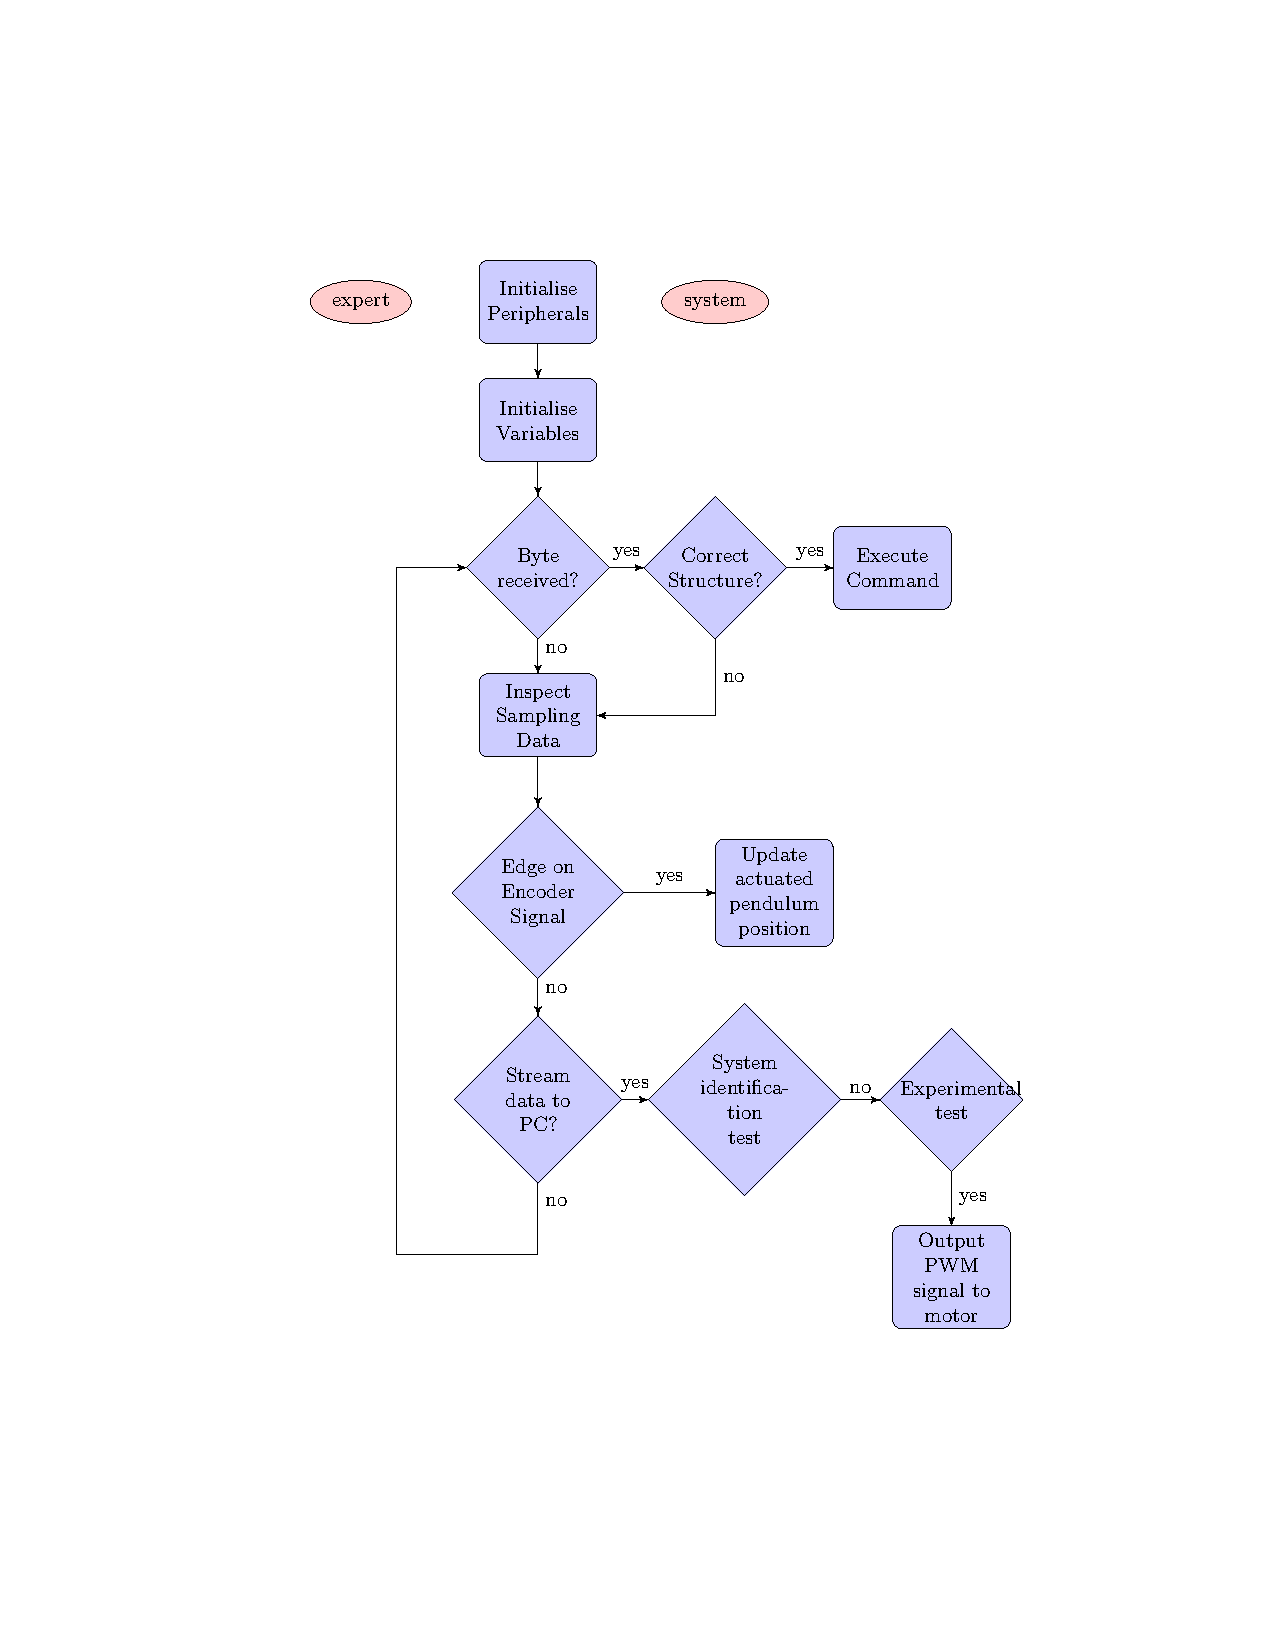
\includegraphics[scale=0.8]{./figs/software_flow/software_flow.pdf}
\caption{Embedded Software Flow}
\label{fig:software_flow}
\end{figure}


Figure \ref{fig:software_flow} shows the main execution flow of the microcontroller based on factors that influence their states. A brief overview of the execution flow is described below.\\

On startup of the microcontroller, the various peripherals required for operation are initialised. They include timers for PWM generation, ADC for sampling and interrupts for encoder signals. The microcontroller will then initialise the various variables required for operation.\\

Once initialisation was completed the microcontroller will check via an interrupt if a byte over the serial communication has been received. If a byte has been received, the microncontroller will verify the command structure and execute based on this command.\\

Every 0.1ms the microcontroller will inspect the data arrays of the sampled signals. Direct Memory Access (DMA) was used for sampling and this results in the sampled data to be automatically refreshed by hardware.\\

The microcontroller will then react whether an interrupt has occured to indicate a rising or falling edge on the encoder signal. This falling and rising edge indicates an incremental change of the position of the actuated pendulum and the microcontroller will behave accordingly.\\

The microcontroller will then verify whether it is required to stream the data every 4ms to the external computer for system identification tests.\\

\subsection{Controller}
%WHAT you are going to present in this chapter/section
%WHY you are presenting it, and
%HOW you are going to present it
The controllers of the swing-up and balancing are implemented on the external computer in a \textit{Python} script and required more information about the system state than what was received from the microcontroller. How this missing information was determined is explained the following section.\\

The information the swing-up and balancing controllers required was the angular velocity of both the actuated and unactuated pendulum. This information was acquired using numerical differentiation by using the 3-point backwards method shown in equation (\ref{eq:differentiation}).

\begin{equation} \label{eq:differentiation}
f'(x) \approx \frac{-3f(x)  +  4f(x-{\Delta}t)  -  f(x-2{\Delta}t)}{ 2{\Delta}t }
\end{equation}

The swing-up controller implements multiple cosine and sine functions. These functions were discretised into a lookup table up to the accuracy provided by the sensors. The discretisation was done to decrease the processing time done to compute the next control input command.


